%%%%%%%%%%%%%%%%%%%%%%%%%%%%%%%%%%%%%%%%%
% University/School Laboratory Report
% LaTeX Template
% Version 3.1 (25/3/14)
%
% This template has been downloaded from:
% http://www.LaTeXTemplates.com
%
% Original author:
% Linux and Unix Users Group at Virginia Tech Wiki 
% (https://vtluug.org/wiki/Example_LaTeX_chem_lab_report)
%
% License:
% CC BY-NC-SA 3.0 (http://creativecommons.org/licenses/by-nc-sa/3.0/)
%
%%%%%%%%%%%%%%%%%%%%%%%%%%%%%%%%%%%%%%%%%

%----------------------------------------------------------------------------------------
%	PACKAGES AND DOCUMENT CONFIGURATIONS
%----------------------------------------------------------------------------------------

\documentclass{article}

\usepackage{siunitx} % Provides the \SI{}{} and \si{} command for typesetting SI units
\usepackage{graphicx} % Required for the inclusion of images
\usepackage{amsmath} % Required for some math elements 
\usepackage[left=1in,top=1in,right=1in,bottom=1in]{geometry}
\usepackage[T1]{fontenc}
\usepackage{verbatim}
\usepackage{setspace}
\usepackage{hyperref}

\setlength\parindent{24pt}

%\usepackage{times} % Uncomment to use the Times New Roman font

%----------------------------------------------------------------------------------------
%	DOCUMENT INFORMATION
%----------------------------------------------------------------------------------------

\title{\bf{Robot Operation via Natural Voice Control}} % Title

\author{Vincent Lee, Calvin Ly, Benjamin Chen\\} % Author name

\date{\today} % Date for the report

\begin{document}

\maketitle % Insert the title, author and date

\onehalfspacing
\begin{center}
\begin{tabular}{l r}
Instructor: & Professor Jivko Sinapov
\end{tabular}
\end{center}

\begin{center}
\begin{tabular}{l r}
\url{https://www.github.com/williewillus/VoiceBot}
\end{tabular}
\end{center}


% Each section should be about one page


\section{Abstract}
In this paper we present an introductory implementation of a natural language movement input system for the BWI robots. The objective is to implement simple and intuitive voice commands as a basic interface for human-robot interaction. The need for this interface arises from the desire to eventually create autonomous, intelligent, robots that can perform a multitude of tasks. These robots have to be capable of carrying out orders from humans through some form of input. Besides the most common input source, vision, audio presents a broad interface that can be used to gather information from the environment. We will present a simple proof-of-concept of such an interface. This interface is built through the use of pocketsphinx, an open-source library created by Carnegie Mellon University that works as a speech recognizer. Phrases are parsed into basic commands (a command language that we have defined for the sole purpose of this endeavor) that the robot can then execute.

\section{Introduction}
In media, robots are portrayed as intelligent beings -- ones that can perfectly understand natural language, and can respond to questions and commands just as a human would. They would be able to blend into society as humans, if not for their electronic innards. This depiction of robots is quite far into the future. For many researchers, this is still the ultimate goal. Small incremental steps have been paved and built upon to reach our status today. Current research focuses mainly on the topics of machine vision, machine learning, navigation, localization, and embodiment.\par

\vspace{5mm}

\noindent We chose to focus on a small yet integral sub-problem of developing intelligence in robots: creating a simple interface to enable human-robot interaction, specifically using speech commands to direct robot movements. Consumer-oriented robots differ from the industrial robots commonly used in manufacturing plants. They are not programmed to do specific tasks with acute attention to detail but rather general tasks adaptable to changing environments. The robot commands must be natural, to be easily operated by humans and the general public, yet logical, for the robot to interpret the intended meaning of the command. These two factors were the basis for our approach to this project.  We first implemented the lowest level base commands possible, turn and move, and then implemented compound commands, dance and spin, to illustrate how higher level abstractions are straightforward with our parser.

\section{Background and Related Work}
Natural language processing is a huge field of research in computer science. Even though human language is constantly changing and evolving, we are able to understand each other. The miracle of how our brains adapt is what the field strives to understand and implement in technology. In this project, we split up natural language processing into two parts: text-to-speech and parsing.\par

\vspace{5mm}

\noindent One resource that we referenced was \textit{Foundations of Statistical Natural Language Processing}. This textbook establishes base knowledge of how researchers approach natural language processing. Furthermore, it outlined issues with the ambiguities and irregularities of language that poke holes in conventional analytical techniques. This gave us ideas of how to structure our commands to be easily parsed by the program. By regulating the form of the command, we can eliminate unintended and misunderstood commands or fill in default information where it is safe to do so. However, at the same time, we lose generality and make the program less forgiving and more frustrating for users. For our purposes, this trade-off is acceptable but may need to be revisited later for future use.\par

\vspace{5mm}

\noindent Additionally, another challenge presented by \textit{Dynamic Programming Algorithm Optimization for Spoken Word Recognition} to natural language processing is the variance in the pace of each person's speech. What was important to understand about this paper was not simply the issue of pacing that it brought up but the fact that speech has so many variables that change from person to person. This makes speech-to-text interpreters incredibly difficult and inconsistent with our current understanding of natural language.\par

% Code descriptions, probably extend this over one page and shorten the prior or next sections
\section{Technical Approach}

\subsection{Overview}
The project is implemented using the ROS Indigo Python platform. Python 2.7 was the language of choice because it is the required language for the RosPy platform, which itself is required by the pocketsphinx library. The entire package is named \texttt{voicebot} (note the casing), and consists of the singular node \texttt{move\_base\_voice.py}, which provides all functionality translating raw audio input into commands to drive the robot's Segway base.

\subsection{Pocketsphinx}
Pocketsphinx is a binding for the CMU Sphinx Natural Language Processing library, written in C.
We use a further specialization of pocketsphinx, \texttt{ros-indigo-pocketsphinx}, that wraps around the original pocketsphinx with a Python and gstreamer binding. This ROS node abstracts away the details of retrieving audio from a microphone device, passing it through Sphinx, and publishing it in String form to a ROS topic (message channel).\par

\vspace{5mm}

\noindent Though this pretty abstraction is convenient for the purposes of our project, we aimed to understand fully how pocketsphinx actually generates String text from raw audio input. This is described on the Sphinx website and we paraphrase here in brief for the reader's convenience.\par

\vspace{5mm}

\noindent Speech, at its core, is simply just a stream of sounds. Language is the ability to segment that sound into discrete units that carry meaning. Although humans are able to learn and reinforce this skill their entire lives, computers are relegated to simply analyzing the incoming data quantitatively. Currently, Sphinx simply detects regions of (relative) silence and splits the audio into words based on that analysis. As you can imagine, this causes it to have some trouble with actual English, which is actually quite slurred in practice.\par

\vspace{5mm}

\noindent First, Sphinx divides the speech into \textit{frames}. From each frame Sphinx calculates a 39-dimension \textit{feature vector}, something that uniquely identifies the speech that was made. Then, this feature vector is fitted to pregenerated model vectors. The closest matching is then elected as the detected word.\par

\noindent One caveat of this approach is immediately seen - we must know all potential words we have to recognize beforehand. Indeed, we had to visit a website and provide it with a list of all possible words we wanted to recognize \footnote{An example of ours can be seen here: \url{https://raw.githubusercontent.com/williewillus/VoiceBot/master/words.sent}}. Then, the website would generate model vector files for those words for pocketsphinx to use.

\subsection{ROS Components}
The full ROS network of our project is very simple. Our node, \texttt{move\_base\_voice}, interfaces with the Segway base using a ROS service client. It receives String inputs from the recognizer by subscribing to the topic \texttt{/recognizer/output}, which pocketsphinx publishes recognized words to.

\begin{figure}[h]
\caption{Subgraph of the RQT Graph for our project}
\centering
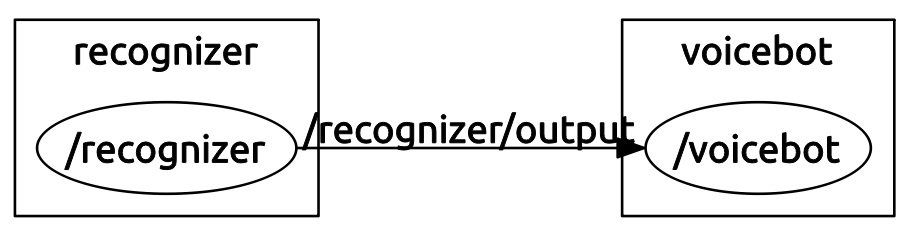
\includegraphics[width=0.5\textwidth]{graph}
\end{figure}

\subsection{Full Implementation Specification}
The ROS node is implemented wholly within one file, \texttt{move\_base\_voice.py}. The class contains one \_\_main\_\_ function. This function first initializes the node with the ROS core, then it creates an actionclient to talk to the Segway base. Then, it instantiates an object of class \texttt{move\_base\_voice}. Instantiating the object subscribes the object's \texttt{speechCb} method to the \texttt{pocketsphinx} recognizer output. Therefore, \texttt{speechCb} will be called whenever \texttt{pocketsphinx} detects any words. After instantiating the object, the main function then enter a spin loop, polling goal tasks from a queue and sending them to the Segway base using the \texttt{actionclient}. The reasoning for using such a queue is explained below. \par

\subsubsection{speechCb}
When the speech callback first receives a string, it first splits the string completely apart using the default Python \texttt{string.split()}. This splits the string into a list of other strings based on any whitespace present, stripping leading and trailing whitespace. Doing this provides us a solid base for beginning parsing. First, if the list resulting from the split is empty, meaning the message consists completely of whitespace, we abort. Then, we test the first word of the list.\par

\vspace{5mm}

\noindent If the first word is "move", and the length of the whole list is 1, then we abort, since there is no meaningful command that can be constructed from just the word "move". Then, we test for a direction in the next word, "forward" or "backward". If neither of those two words are present, "forward" is assumed. Then, we see if there are any more words. If not, then we simply have the command "move forward" or "move backward", and assume that that means 1 meter in the corresponding direction. Following that, the more complicated part of the parsing begins. We call a utility function that scans through a sublist of the split list from the first word that isn't "move" or "backwards" or "forwards" until the end of the list. It returns two values: its attempt to parse an integer out of the list's words, and the first index of a non-number word that it encountered and terminated on.
Then, we pick up from that index and attempt to find a unit, one of "foot", "feet", "meter", "meters", "inch", or "inches". If none is provided, "meters" is assumed. Otherwise, the appropriate unit conversions are applied to convert the respective unit into meters, the Segway base's native measurement unit. If moving backward, first \texttt{speechCb} itself is called with "turn left one hundred eighty degrees". This demonstrates the flexibility of the callback in its ability to compose commands out of other commands. Finally, it creates a \texttt{MoveBaseGoal} object out of the meter distance and appends it to the queue. \par

\vspace{5mm}

\noindent The "turn" command works in nearly an identical way as the move command. There are several key differences. First, "left" and "right" are used instead of "forward" and "backward". Turning right multiplies the turn angle by -1 instead of sending a separate command like moving. The detected units are "radians" and "degrees", defaulting to "90" and "degrees" if the amount or unit are not present, respectively. The encoded \texttt{MoveBaseGoal} object also represents a quaternion rotation instead of a linear motion. Special care was taken here to normalize the quaternion here to 1, which is the identity quaternion, instead of leaving them at their default values of 0. Doing that would result in the action client erroring out from an invalid rotation.\par

\vspace{5mm}

\noindent The "spin" command simply calls \texttt{speechCb} again with "turn left one hundred eighty degrees" 100 times. Again this shows the flexible way we can compose commands out of other commands.\par

\vspace{5mm}

\noindent The "dance" command executes a sequence of moves drawing some sort of fractal-flower shape on the ground, again composing itself out of other commands. This usually doesn't work in enclosed spaces, as the base's obstacle avoidance code will modify the actual path taken.

\vspace{5mm}

\noindent The "stop" command is unique. Upon receiving this command, the goal queue is immediately cleared, stopping any and all ongoing spins and dances. This is also why we opted to implement a goal queue instead of having all commands directly message the base. By using a queue, stop can be implemented by simply clearing the queue, instead of having to interrupt other threads' invocations of \texttt{speechCb}

\subsubsection{try\_parse\_number}
The utility function mentioned above is adapted from a post on StackOverflow (cited below). The original code sample simply provides a primitive way to parse the string representation of a number into an actual numerical value. It does this by filling the appropriate positions of an array with the strings and then creates a dictionary from number words to numerical values. The string is then scanned by looking each word up and multiplying/adding the values into some accumulator. We modify the function to also return the index of the first unrecognizable word, for the purposes cited above.

\subsection{Implemented Commands}
\begin{itemize}
    \item Move <x> $\Rightarrow$  Move <x> meter
    \item Move <x> <foot | feet | inch | inches | meter | meters>
    \item Move forward $\Rightarrow$ Move 1 meters
    \item Move backward $\Rightarrow$ Turn 180 degrees; move 1 meters
    \item Turn right $\Rightarrow$ Turn -90 degrees
    \item Turn left $\Rightarrow$ Turn 90 degrees
    \item Turn <x> $\Rightarrow$ Turn <x> degrees
    \item Turn <x> <radians | degrees>
    \item Spin $\Rightarrow$ Turn 180 degrees
    \item Dance $\Rightarrow$ Executes a dance
    \item Stop $\Rightarrow$ Clear all queued commands (mostly to stop disaster in testing, and to stop spin and dance)
\end{itemize}
 

\section{Experiments and Evaluations}
To test our proof-of-concept for correctness, we used a combination of white-box and black-box testing on the robots in the lab. The audio parsing itself was primarily tested by using \texttt{rostopic echo} to see what goals were published to the \texttt{move\_base\_client}. By checking to see if the position and orientation were correct for their respective commands, we were able to determine that our program sent the correct commands to the robot base.\par

\vspace{5mm}

\noindent For the overall execution of the program, we tested on the actual BWI robots in the lab. The robot was given voice commands to execute and we checked to see if it moved accordingly. Through this method we were able to determine that our program was working as intended. We ran into several initial challenges:
\begin{itemize}
    \item The robot cannot directly move backwards because it has no obstacle collision avoidance at the rear end. This problem was solved by simply turning one hundred eighty degrees and then moving forward, but relies on the accuracy of the turning to effectively move backwards.
    \item The microphone quality greatly affects the accuracy of the voice recognizer
    \item The orientation quaternion needs to be normalized to 1, even though the default quaternion is 0
    \item The area that we tested in was too narrow to properly test some of the commands, such as dance. 
\end{itemize}

\section{Future Work}
\subsection{User response}
Currently, an invalid command results in, effectively, a no-op instruction. The robot could eventually be programmed to give informative and helpful error responses whenever an invalid command is attempted. For example, a command that begins with a unit of measurement could be interpreted as "NO ACTION GIVEN" and could report that the user.
\subsection{Additional commands}
The robots we tested our program on can only move forward and turn. The low-level commands are limited by the robot's range of motion. On a robot with more moving parts, we could implement even more commands. On a robot with arms we could implement commands such as grasp, contract elbow, rotate wrist, and other commands for each joint that moves. Higher-level commands could then be implemented using these new commands.
\subsection{Higher-level commands}
Commands that are more useful to humans (in the case of a general-use robot) could be implemented in the future, especially as navigation, machine vision, and localization improve. Commands such as "pickup [object]", "go to [location]", or "follow [object/person]". These higher-level commands will simply use a combination of lower-level commands (move, turn, etc) and current navigation/localization and machine vision to execute.
\subsection{Intelligent deduction of commands}
The robots could include some sort of command context, where the robot is aware of commands that have been issued in the past. For example, if a human issues a sequence of commands and then says "Return to starting position", the robot would know to return to the very first initial pose. Or, if a human stands in front of the robot and says "Come here", the robot should know to navigate to the human. This borders on the edge of other forms of artificial intelligence, and could take advantage of technology from consumer companies like Apple's Siri, Microsoft's Cortana, or Google Now. It would also require more advanced sensing and hardware to detect the directional source of the input.
\subsection{Improved Audio Detection}
Our current implementation relies on \texttt{pocketsphinx} for speech recognition. This, however, limits our project in various ways. A dictionary of possible words must be defined, and as the dictionary gets larger, the audio parsing becomes less accurate. With an improved method of audio parsing, commands could be executed more robustly and the robot operation would be much more smooth. The command language could also be more flexible with a better speech recognition engine, if it was not restricted by the need for a dictionary of possible words. One problem we encountered while working was that some words would be misinterpreted. The word "turn' kept being interpreted as the word "two".

\section{Conclusion}
Human-robot interaction cannot be done without some sort of interface linking the two together. In this paper
we have presented a simple and working proof-of-concept implementation of a basic human-robot interface system using voice commands. While not the most polished, it illustrates that building this interface can be relatively straightforward and effective with the amount of resources that are widely available now. The robot can understand natural language in a limited sense and then execute commands based what it hears.\par

\vspace{5mm}

\noindent However, what we have presented is only a basic example of communication between robots and humans. There is no true understanding of the commands in the robot. As the field of autonomous intelligence in robots grows, we hope to achieve this true understanding.

\section{Sources Cited}
\begin{itemize}
    \item A numerical parsing implementation. (n.d.). Retrieved May 11, 2016, from \url{http://stackoverflow.com/a/493788}.
    \item CMUSphinx. (n.d.). Retrieved May 11, 2016, from \url{http://cmusphinx.sourceforge.net/wiki/} 
    \item PocketSphinx. (n.d.). Retrieved May 11, 2016, from \url{http://wiki.ros.org/pocketsphinx}
    \item H. Sakoe and S. Chiba, "Dynamic programming algorithm optimization for spoken word recognition," in IEEE Transactions on Acoustics, Speech, and Signal Processing, vol. 26, no. 1, pp. 43-49, Feb 1978.
doi: 10.1109/TASSP.1978.1163055
    \item Manning, C. D., \& Sch\"{u}tze, H. (1999). Foundations of statistical natural language processing (Vol. 999). Cambridge: MIT press.
\end{itemize}

\end{document}
